% Lulu.com Cover Template
% This template creates a single-page PDF with: Back Cover + Spine + Front Cover
% 
% Dimensions configured for: 380-page, 6"x9" book
% Total dimensions: 14.875" x 10.75" (from Lulu.com)
% Spine width: 1.125"

\documentclass{article}
\usepackage{xcolor}
\usepackage{graphicx}
\usepackage{tikz}
\usepackage{textpos}
\usepackage{fontspec} % For better font handling (requires XeLaTeX or LuaLaTeX)
% If using pdflatex, use: \usepackage[T1]{fontenc}

% ============================================
% PAGE SETUP
% ============================================
\usepackage[paperwidth=14.875in,paperheight=10.75in,margin=0pt,noheadfoot]{geometry}
\pagestyle{empty}

% Force exact page dimensions
\pdfpagewidth=14.875in
\pdfpageheight=10.75in

% ============================================
% COVER CONTENT
% ============================================

\begin{document}
\thispagestyle{empty}
\setlength{\parindent}{0pt}
\setlength{\parskip}{0pt}

% Use TikZ with absolute positioning from page corners
\begin{tikzpicture}[remember picture,overlay,x=1in,y=1in]
  % Back Cover (left side: full height from bottom-left corner)
  \node[anchor=south west,inner sep=0] at (current page.south west) {
    
\includegraphics[width=6.875in,height=10.75in,keepaspectratio=false]{assets/interfaces_backcover.jpg}
  };
  
  % Back cover text overlay - using textblock for better text flow
  % Position text block starting from top-left, with margins
  \begin{scope}[shift={([xshift=0.55in]current page.south west)}]
    % Title at top
    \node[anchor=north west,text width=5.775in,align=center,text=black] 
      at (0,10.2in) {
      {\Large\textbf{Interfaces of Reality}}\\[0.3\baselineskip]
      {\textit{How Life, Mind, and Machines Navigate a World of Possibilities}}\\[1\baselineskip]
    };
    
    % Main description text - part 1
    \node[anchor=north west,text width=5.775in,align=left,text=black,font=\small] 
      at (0,8.8in) {
      \textbf{What if everything you thought you knew about reality is incomplete?}\\[0.4\baselineskip]
      
      For centuries, we've believed the universe is made of things, particles, atoms, molecules, cells. But this view cannot explain the deepest mysteries: Why do eyes evolve the same design independently, across millions of years? How does a cell remain itself when every molecule is replaced? Why do AI systems, trained separately, discover identical structures for language and vision? What makes you \textit{you}, even as your body completely renews itself?\\[0.4\baselineskip]
      
      \textbf{The answer lies not in the things themselves, but in the boundaries between them.}\\[0.4\baselineskip]
      
      In this groundbreaking work, systems architect and researcher Stephane Fellah reveals a radical new way of seeing reality. Drawing from cutting-edge discoveries in physics, biology, artificial intelligence, and his own pioneering work in semantic technologies, he shows that reality is not fundamentally made of objects, but of \textit{stable interfaces}, boundaries that constrain interaction while enabling persistence.\\[0.4\baselineskip]
      
      Once you see interfaces, they appear everywhere: in the membrane of a cell, the structure of a mind, the design of a machine, the patterns of meaning. The same principles that create atoms also create meaning. The same boundaries that make cells stable also make AI systems intelligent. This is not coincidence, it is the deep structure of reality itself.
    };
    
    % Central claim box - positioned lower
    \node[anchor=north west,text width=5.775in,align=center,text=black,font=\small]
      at (0,5.2in) {
      \fbox{\begin{minipage}{5.375in}
      \vspace{0.4\baselineskip}
      \begin{center}
      {\Large\textbf{THE CENTRAL CLAIM}}\\[0.4\baselineskip]
      \end{center}
      \textit{Reality is not fundamentally made of things, but of stable interfaces navigating a structured space of possibilities.}
      \vspace{0.4\baselineskip}
      \end{minipage}}
    };
    
    % Main description text - part 2
    \node[anchor=north west,text width=5.775in,align=left,text=black,font=\small]
      at (0,4.1in) {
      \textbf{You will never see the world the same way again.}\\[0.4\baselineskip]
      
      From the quantum realm to artificial intelligence, from the birth of life to the nature of consciousness, \textit{Interfaces of Reality} offers a unifying perspective that transforms how we understand matter, mind, machines, and meaning. This is not just a new theory, it is a new way of seeing, one that reveals the hidden architecture holding our universe together.
    };
    
    % Author bio at bottom
    \node[anchor=south west,text width=5.775in,align=left,text=black,font=\scriptsize] 
      at (0,1.0in) {
      \textbf{About the Author}\\[0.3\baselineskip]
      
      Stephane Fellah is a systems architect, researcher, and entrepreneur who has spent decades working at the frontier of artificial intelligence, semantic technologies, and geospatial systems. His fascination with the deep structure of reality began during his studies in physics and mathematics in France, where he was captivated by the elegance of physical laws and the persistent question: \textit{Why are the laws structured this way?}\\[0.3\baselineskip]
      
      As an ontologist building systems that bridge logic and reality, and as someone who has witnessed AI systems independently discover the same structures that evolution found, Fellah recognized a profound pattern: the same principles govern everything from atoms to minds. \textit{Interfaces of Reality} is the result of that synthesis, a journey from wonder to practice to understanding, revealing the hidden architecture that makes our universe possible.
    };
  \end{scope}
  
  % Spine (center: positioned from bottom-left, starting at 6.875 inches)
  % Use beige color to match the cover
  \definecolor{coverbeige}{RGB}{245,245,220}  % Beige color
  \fill[color=coverbeige] ([xshift=6.875in]current page.south west) 
    rectangle ([xshift=8.0in,yshift=10.75in]current page.south west);
  
  \node[rotate=90,anchor=center,text=black,font=\fontsize{24}{28}\selectfont\bfseries] 
    at ([xshift=7.4375in,yshift=5.5in]current page.south west) {
    Interfaces of Reality
  };
  
  \node[rotate=90,anchor=center,text=black,font=\fontsize{14}{16}\selectfont] 
    at ([xshift=7.4375in,yshift=3.0in]current page.south west) {
    Stephane Fellah
  };
  
  % Front Cover (right side: starts at 8.0 inches from left edge, full height)
  \node[anchor=south west,inner sep=0] at ([xshift=8.0in]current page.south west) {
    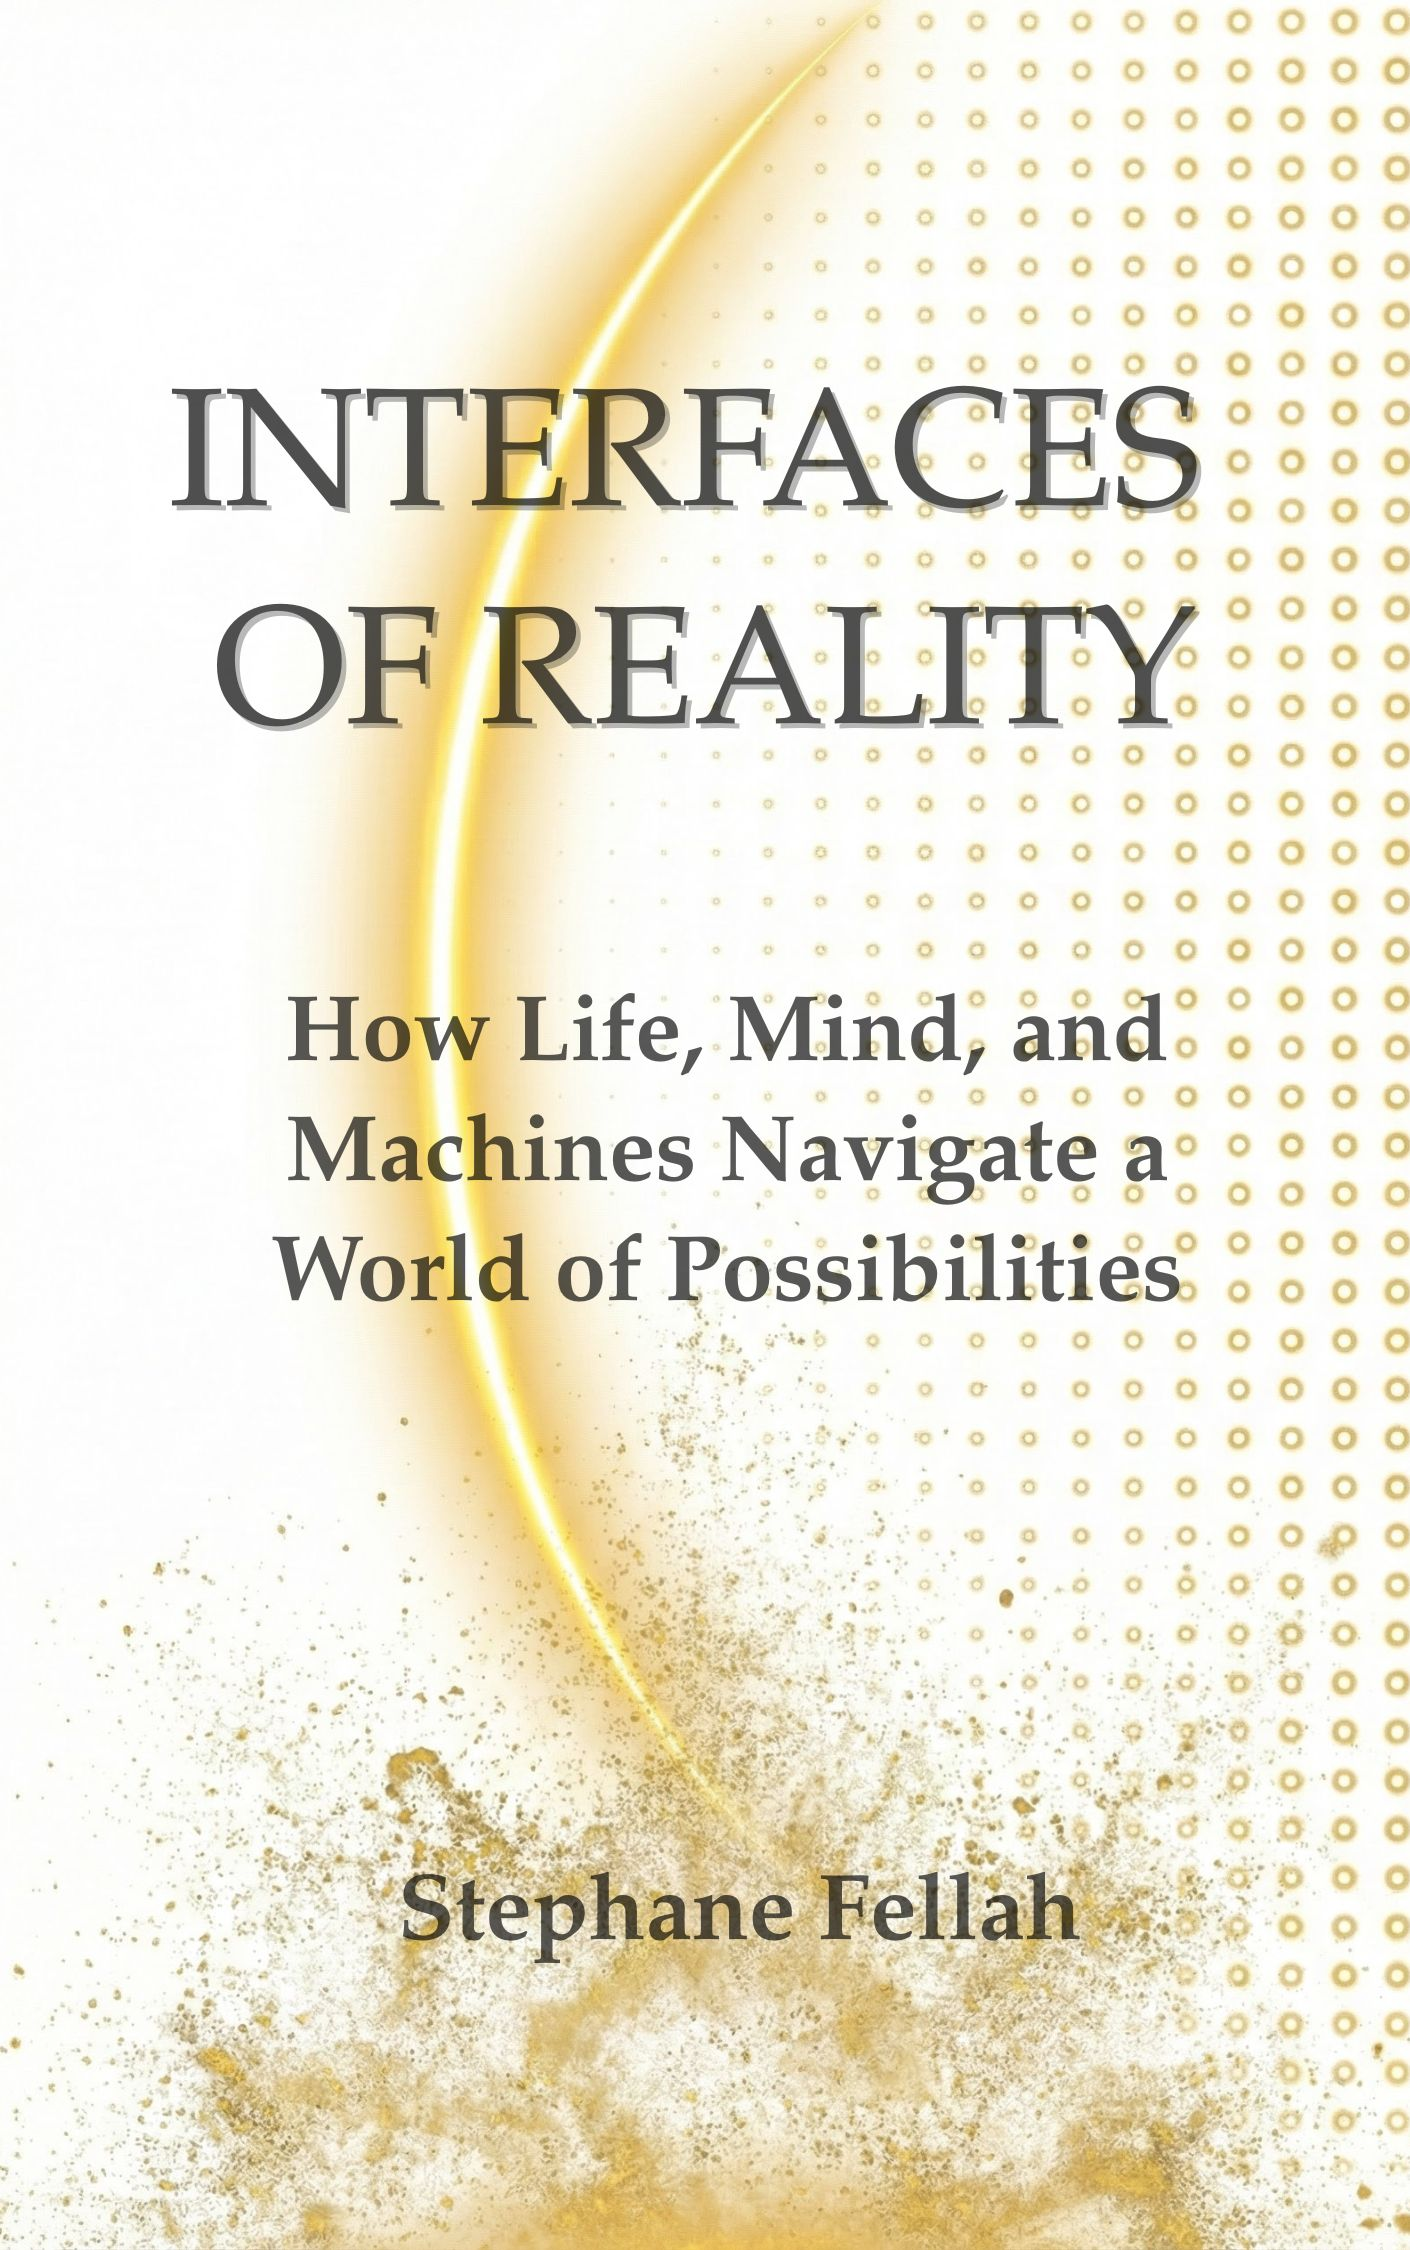
\includegraphics[width=6.875in,height=10.75in,keepaspectratio=false]{assets/front-page.jpg}
  };
  
\end{tikzpicture}

\end{document}
